\subsection{Optimizavimo algoritmo įtaka}
\label{subsec:rez_optimizatorius}

Lyginami keturi optimizavimo algoritmai: \textit{Adam}, \textit{AdamW}, \textit{RMSprop} ir \textit{SGD} (be momentumo). Visų algoritmų \texttt{learning\_rate}~$=10^{-3}$. Rezultatai pateikti~\ref{tab:rez_optimizatorius} lentelėje, validavimo metrikų kitimas – \ref{fig:rez_optimizatorius_image} ir~\ref{fig:rez_optimizatorius_keystroke} pav.

\begin{table}[H]
    \centering
    \caption{Optimizavimo algoritmo tyrimo rezultatai. Geriausi variantai paryškinti.}
    \begin{tabular}{|l|l|c|c|c|}
        \hline
        Užduotis & Algoritmas & \texttt{val\_acc} & \texttt{val\_loss} & \texttt{test\_acc} \\
        \hline
        \multirow{4}{*}{Vaizdai}
            & \textbf{\textit{Adam}}    & $\mathbf{0{,}8466}$ & $0{,}6524$ & $0{,}8347$ \\ \cline{2-5}
            & \textit{SGD}              & $0{,}5503$ & $0{,}6801$ & $0{,}5424$ \\ \cline{2-5}
            & \textbf{\textit{RMSprop}} & $\mathbf{0{,}8466}$ & $0{,}4883$ & $0{,}8390$ \\ \cline{2-5}
            & \textit{AdamW}            & $0{,}8413$ & $\mathbf{0{,}4512}$ & $\mathbf{0{,}8432}$ \\
        \hline
        \multirow{4}{*}{Laiko eilutės}
            & \textit{Adam}             & $0{,}6708$ & $1{,}1537$ & $0{,}7067$ \\ \cline{2-5}
            & \textit{SGD}              & $0{,}0333$ & $3{,}4034$ & $0{,}0333$ \\ \cline{2-5}
            & \textbf{\textit{RMSprop}} & $\mathbf{0{,}7042}$ & $\mathbf{1{,}1310}$ & $\mathbf{0{,}7300}$ \\ \cline{2-5}
            & \textit{AdamW}            & $0{,}6833$ & $1{,}1355$ & $0{,}7200$ \\
        \hline
    \end{tabular}
    \label{tab:rez_optimizatorius}
\end{table}


\begin{figure}[H]
    \centering
    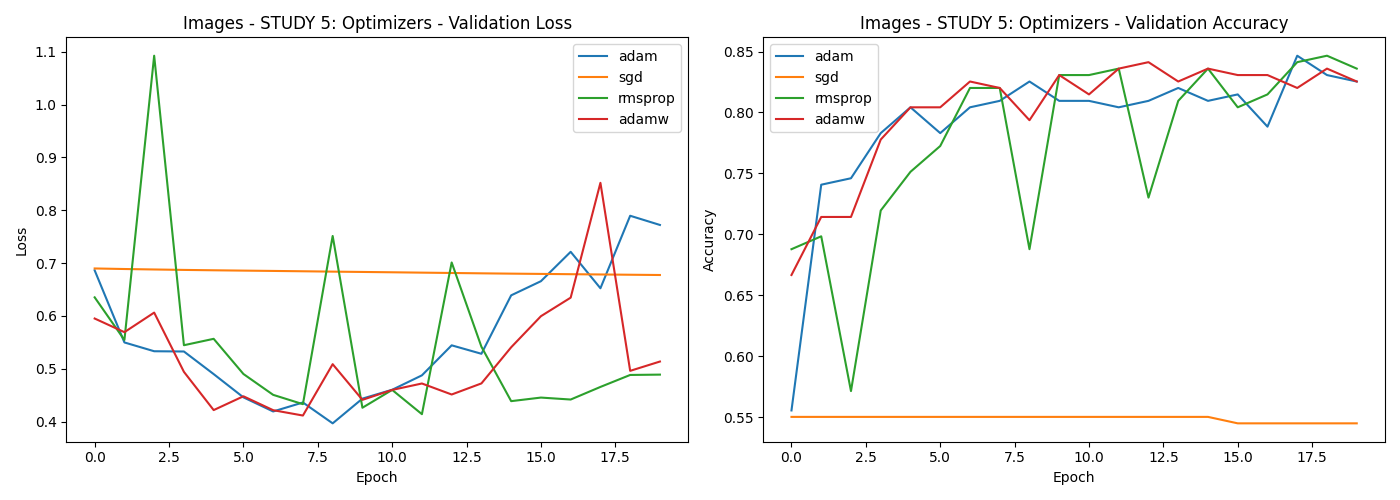
\includegraphics[width=0.9\linewidth]{3Lab/results/optimizer/img_comparison.png}
    \caption{Optimizavimo algoritmo tyrimas – vaizdų užduotis}
    \label{fig:rez_optimizatorius_image}
\end{figure}

\begin{figure}[H]
    \centering
    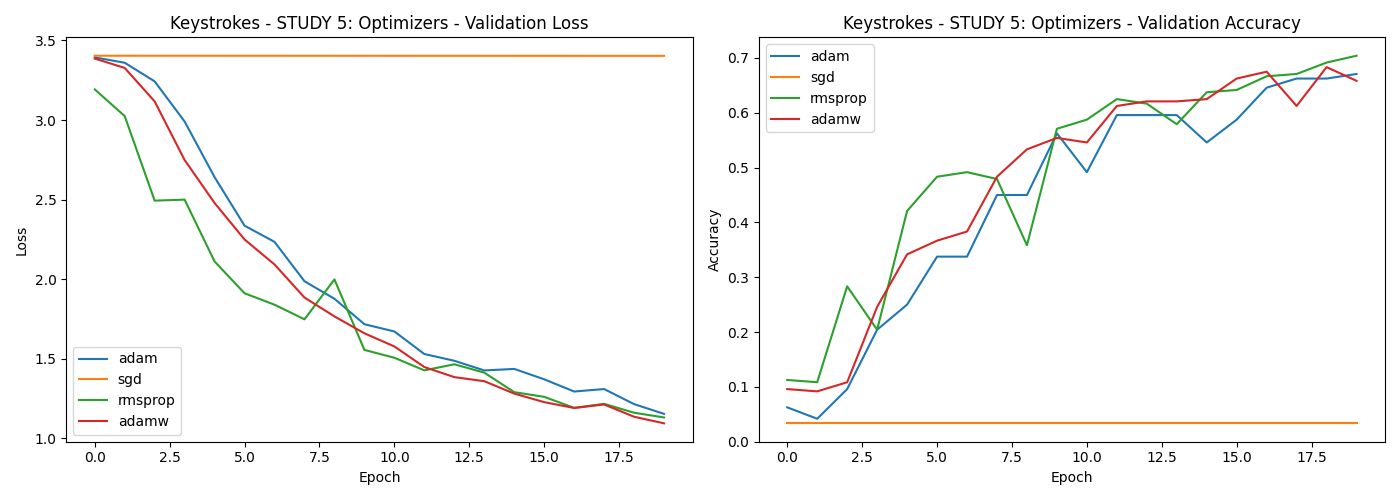
\includegraphics[width=0.9\linewidth]{3Lab/results/optimizer/ks_comparison.png}
    \caption{Optimizavimo algoritmo tyrimas – laiko eilučių užduotis}
    \label{fig:rez_optimizatorius_keystroke}
\end{figure}

Pastebimi rezultatai:
\begin{itemize}
    \item \textit{Adam}, \textit{AdamW} ir \textit{RMSprop} gauna labai panašius rezultatus, nes visi naudoja adaptyvų mokymosi greitį pagal kiekvieno svorio gradiento istoriją.
    \item \textit{SGD} su tokia pačia $10^{-3}$ vertė ryškiai atsilieka – ypač $30$ klasių laiko eilučių užduotyje, kur \texttt{test\_acc}~$=0{,}0333$ (atsitiktinis spėjimas). Kad \textit{SGD} dirbtų konkurencingai, reikėtų paskaičiuoti tinkamą \texttt{learning\_rate} ir/arba pridėti momentumą.
    \item Pagal numatytąsias hiperparametrų reikšmes \textit{Adam} išlieka saugus pasirinkimas abiem užduotims.
\end{itemize}
